\chapter{Einleitung}
\label{chapter:Einleitung}

\section{Motivation der Hyperloop Technologie}
\label{section:Motivation}

Der Hyperloop ist ein innovatives Transportkonzept, das eine ökonomische, klimafreundliche und schnellere Alternative zu herkömmlichen Verkehrsmitteln wie Lastkraftwagen, Zügen und Flugzeugen bietet.\\
\pagebreak[3]
\begin{figure}[!ht]
	\begin{center}
		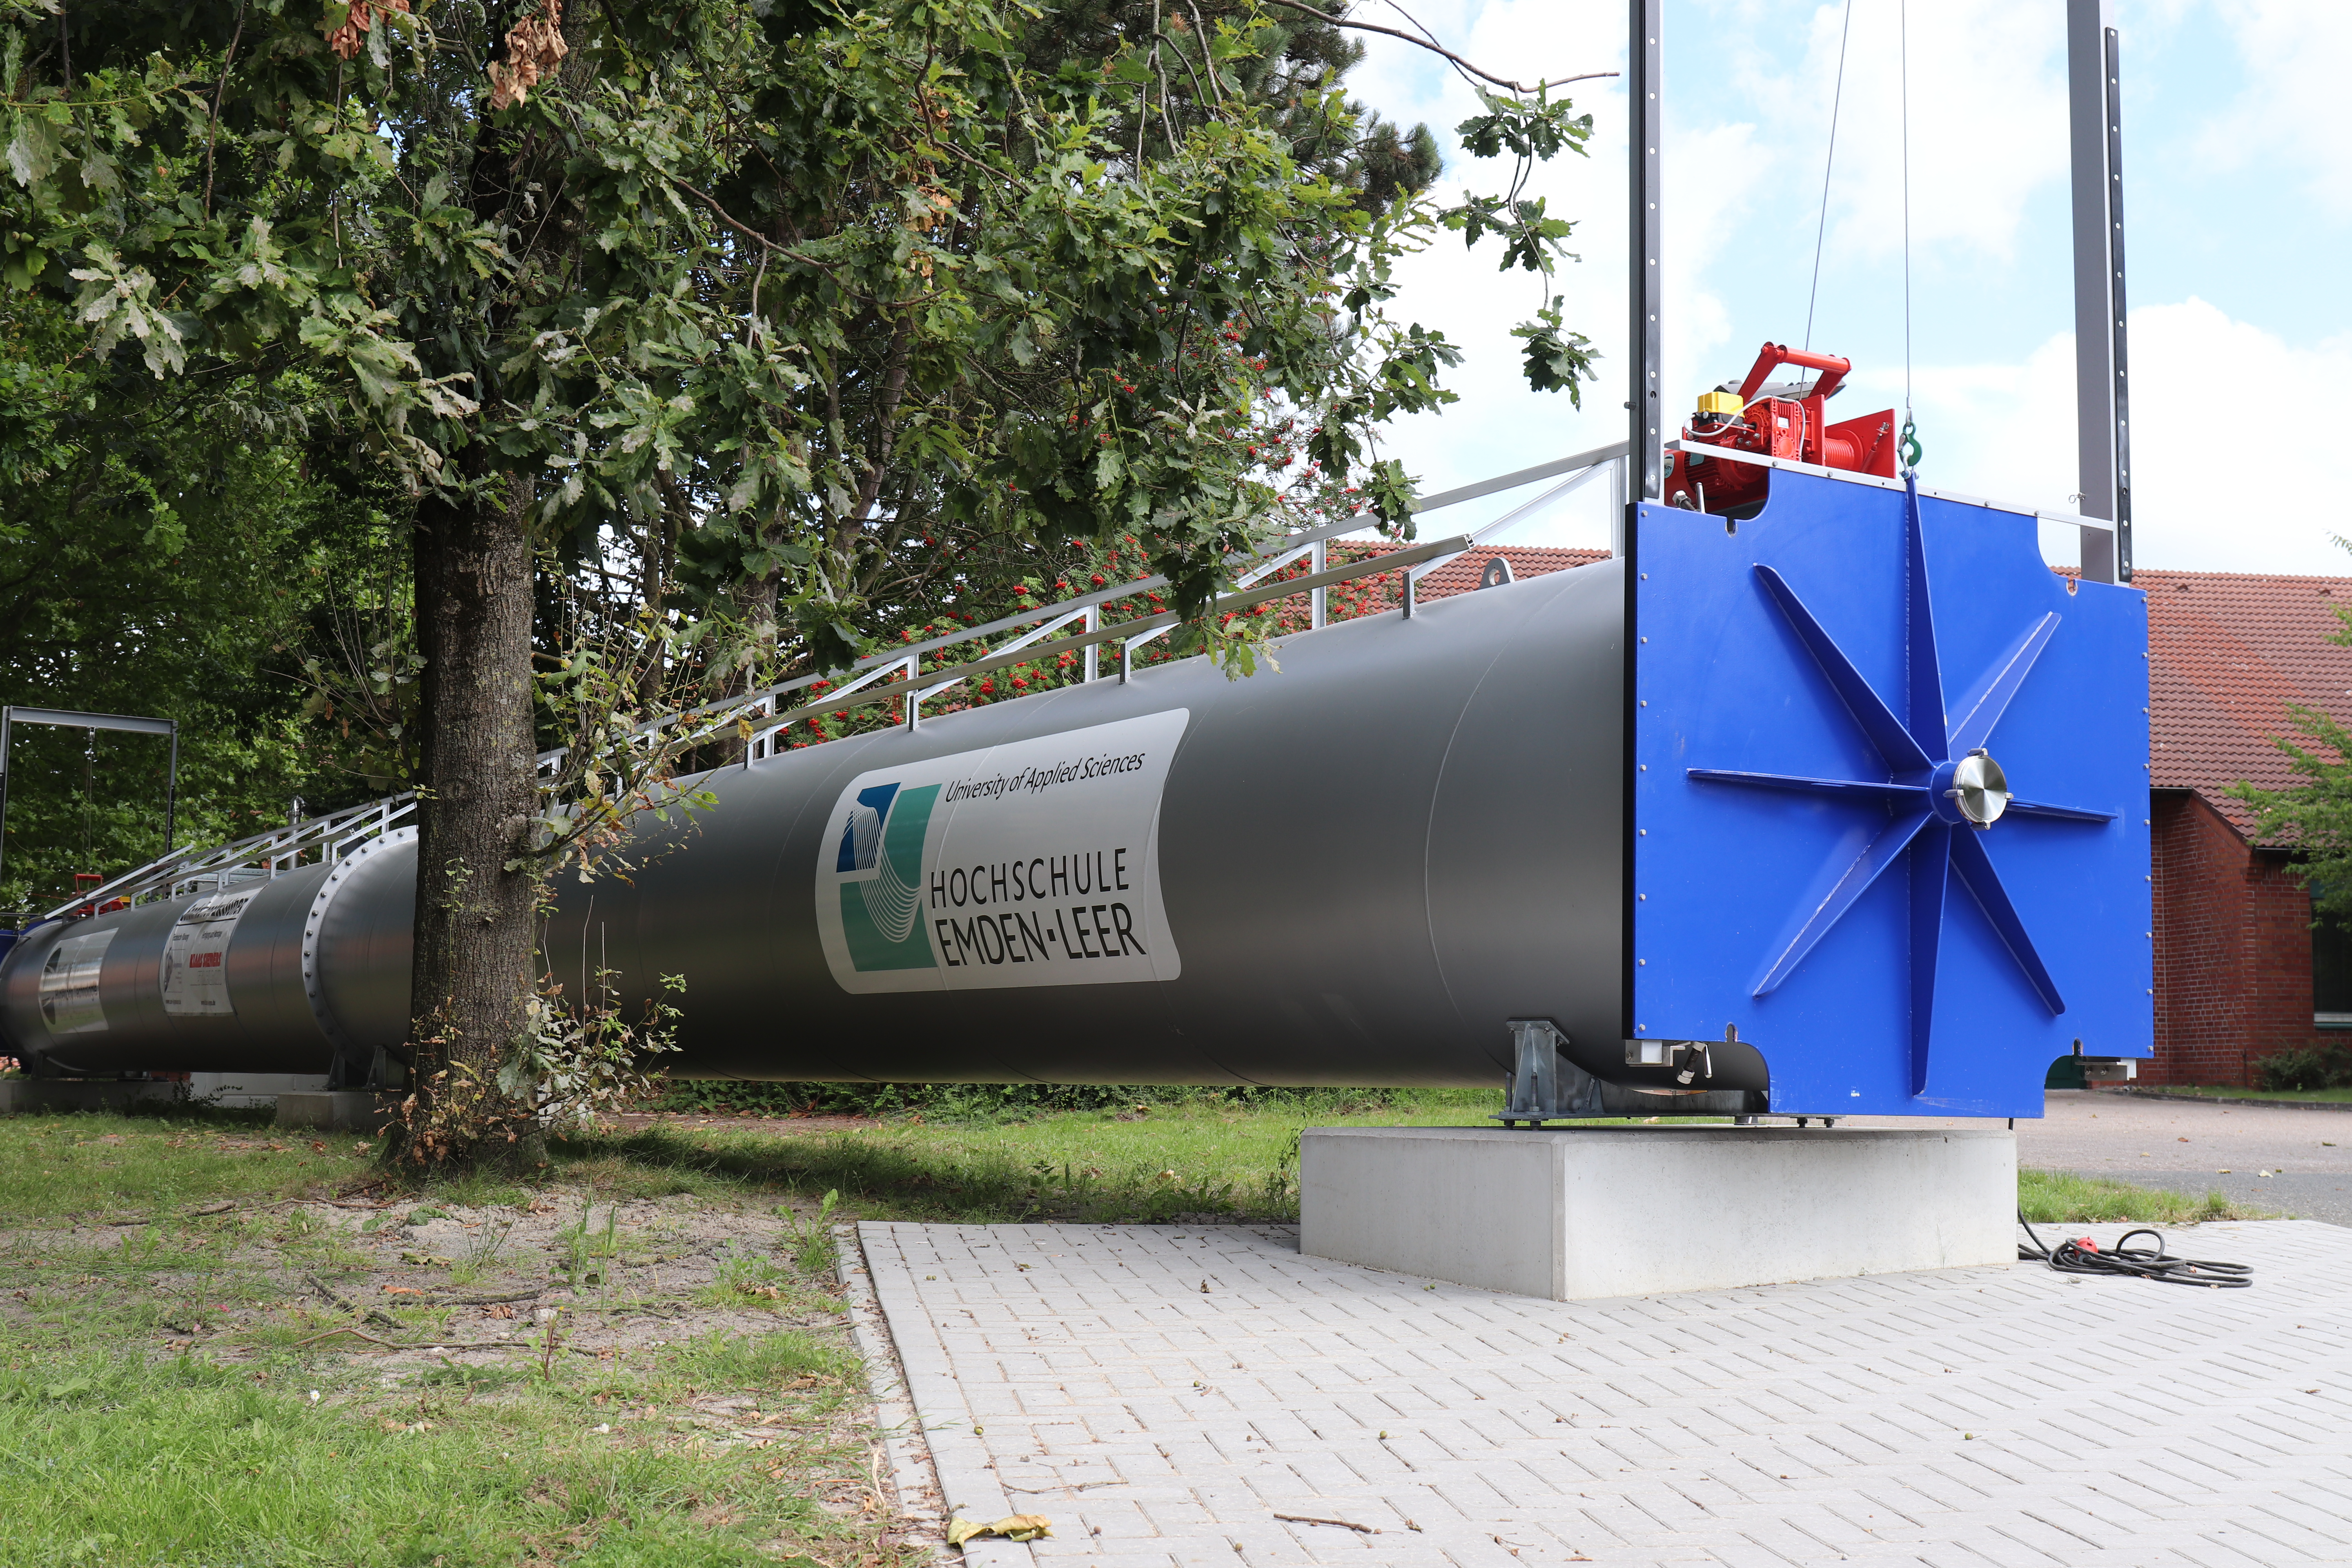
\includegraphics[width=1\textwidth]{img/1_strecke/strecke_1.png}
		\caption{Hyperloop der Hochschule Emden-Leer}
		\label{img_1_1:strecke}
	\end{center}
\end{figure}
\pagebreak[4]
Derzeit stehen herkömmlichen Transportmitteln zwei wesentliche Hindernisse im Weg, um Personen und Güter schnell und emissionsarm zu befördern. Zum einen der hohe Luftwiderstand, der bei hohen Geschwindigkeiten den Energieverbrauch stark erhöht.\\
Der Hyperloop löst diese Probleme, indem er Güter und Personen in einem Fahrzeug, das sich in einer fast Vakuumröhre bewegt, wie in Abbildung \ref{img_1_1:strecke} dargestellt ist.



%%%%%%%%%%%%%%%%%%%%%%%%%%%%%%%%%%%%%%%%%%%%%%%%%%%%%%%%%%%%%%%%%%%%%%%%%%%%%%%%%%%%
%%%%%%%%%%%%%%%%%%%%%%%%%%%%%%%%%%%%%%%%%%%%%%%%%%%%%%%%%%%%%%%%%%%%%%%%%%%%%%%%%%%%
%%%%%%%%%%%%%%%%%%%%%%%%%%%%%%%%%%%%%%%%%%%%%%%%%%%%%%%%%%%%%%%%%%%%%%%%%%%%%%%%%%%%
%%%%%%%%%%%%%%%%%%%%%%%%%%%%%%%%%%%%%%%%%%%%%%%%%%%%%%%%%%%%%%%%%%%%%%%%%%%%%%%%%%%%
%%%%%%%%%%%%%%%%%%%%%%%%%%%%%%%%%%%%%%%%%%%%%%%%%%%%%%%%%%%%%%%%%%%%%%%%%%%%%%%%%%%%
%%%%%%%%%%%%%%%%%%%%%%%%%%%%%%%%%%%%%%%%%%%%%%%%%%%%%%%%%%%%%%%%%%%%%%%%%%%%%%%%%%%%



\subsection*{Institute of Hyperloop Technology}
\label{section:IHT}

%Die Hochschule Emden/Leer hat im Jahr 2021 das Institut für Hyperloop-Technologie (IHT) gegründet, um aktiv an der Forschung zu dieser zukunftsweisenden Technologie teilzunehmen.

Im Rahmen dieser Forschung-arbeit, -projekt wurde an der Hochschule Emden eine Teststrecke mit einer Länge von 27 Metern errichtet (siehe Abbildung \ref{img_1_1:strecke}). Auf dieser Strecke soll das Fahrzeug (Cargo-Pod) unter realistischen Bedingungen getestet und weiterentwickelt werden.
Die Teststrecke besteht aus einem Schienensystem und einem Linearmotor.\\
Die Forschung des \frqq Institute of Hyperloop Technology\flqq, fokuziert sich auf die Güterbeförderung.
\newpage




\section{Aufgabenstellung}
\label{section:Aufgabenstellung}
Das Ziel dieses Projektes ist die Entwilckung eines Hyperloop-Fahrzeuges, das mit einer Batterie und einem Motor betrieben wird. Für die Steuerung des Fahrzeugs wurde ein echtzeitfähiges Steuerungsystem der Firma Speedgoat vorgeben, welches in Abschnitt \ref{section:speedgoat} vertiefend erläutert wird.\\ \ \\

Im Rahmen des Projekts wird ein Fahrzeug (Pod) für den Hyperloop mit einer Bordspannung von 48 V konzipiert. Ziel ist es, die Realisierbarkeit dieser Spannung zu überprüfen und umzusetzen. Dazu gehören die Planung und Simulierung, die Integration der erforderlichen Sensorik sowie die Beschaffung der notwendigen Bauteile. Die Logik- und Signalverarbeitung wird, mithilfe von Simulink, auf dem echtzeitfähigen Speedgoat-System durchgeführt.
Die Steuerung erfolgt über Simulink, ein Modul von MATLAB, und beinhaltet die Erfassung von Position und Beschleunigung des Fahrzeuges. Der Motor wird über ein zusätzliches Steuergerät angesteuert. Die Steuerung soll in Form einer Automatensteuerung umgesetzt werden.
Die Verdrahtung des Pods wird entsprechend der Bordspannung von 48 V ausgelegt. Hierfür wird mit der Software QElectroTech ein Schaltplan (siehe Anhang \ref{Anhang:Schaltplan}) erstellt.
Alle erforderlichen Bauteile für die Umsetzung der Bordspannung, die Verdrahtung und die Sensorik müssen beschafft werden.\\
Textergebnisse und Inbetriebnahme entfallen.


%%%%%%%%%%%%%%%%%%%%%%%%%%%%%%%%%%%%%%%%%%%%%%%%%%%%%%%%%%%%%%%%%%%%%%%%%%%%%%%%%%%%
%%%%%%%%%%%%%%%%%%%%%%%%%%%%%%%%%%%%%%%%%%%%%%%%%%%%%%%%%%%%%%%%%%%%%%%%%%%%%%%%%%%%
%%%%%%%%%%%%%%%%%%%%%%%%%%%%%%%%%%%%%%%%%%%%%%%%%%%%%%%%%%%%%%%%%%%%%%%%%%%%%%%%%%%%
%%%%%%%%%%%%%%%%%%%%%%%%%%%%%%%%%%%%%%%%%%%%%%%%%%%%%%%%%%%%%%%%%%%%%%%%%%%%%%%%%%%%
%%%%%%%%%%%%%%%%%%%%%%%%%%%%%%%%%%%%%%%%%%%%%%%%%%%%%%%%%%%%%%%%%%%%%%%%%%%%%%%%%%%%
%%%%%%%%%%%%%%%%%%%%%%%%%%%%%%%%%%%%%%%%%%%%%%%%%%%%%%%%%%%%%%%%%%%%%%%%%%%%%%%%%%%%

\section{Aufbau der Projektdokumentation}
\label{section:Aufbau}


Die Projektdokumentation beginnt mit einer Einführung in die Hyperloop-Technologie und der Aufgabenstellung dieses Projekts, die die Motivation und Zielsetzungen erläutern. Es wird dargelegt, warum der Hyperloop als innovative, umweltfreundliche Transportlösung eine wichtige Alternative zu bestehenden Systemen darstellt und welche spezifischen Herausforderungen und Ziele mit der Entwicklung eines funktionsfähigen Prototyps verbunden sind.

Im weiteren Verlauf wird das grundlegende Fahrzeugkonzept vorgestellt. Dabei wird beschrieben, wie die verschiedenen Baugruppen miteinander verbunden sind und welche Rolle das zentrale Steuerungssystem von Speedgoat übernimmt. Auch die verwendeten Sensoren und deren Einbindung in das Gesamtsystem werden erläutert.

Der Dokumentationsteil zur Implementierung zeigt die technische Realisierung der Steuerung und der elektrischen Verdrahtung des Fahrzeugs. Die Erstellung des Schaltplans, die Konfiguration der Steuerlogik sowie die detaillierte Beschreibung der Automatik- und manuellen Steuerungsmodi geben Einblicke in die Funktionsweise und den Aufbau des Systems. Ergänzend wird die Integration der Distanzmessung beschrieben, die eine präzise Positionsermittlung innerhalb der Teststrecke ermöglicht.

Abschließend fasst die Konklusion die Ergebnisse der Projektarbeit zusammen und gibt Hinweise auf mögliche zukünftige Entwicklungen. Hierbei wird auch die Offenheit der Systemarchitektur betont, die eine flexible Weiterentwicklung ermöglicht..


%%%%%%%%%%%%%%%%%%%%%%%%%%%%%%%%%%%%%%%%%%%%%%%%%%%%%%%%%%%%%%%%%%%%%%%%%%%%%%%%%%%%
%%%%%%%%%%%%%%%%%%%%%%%%%%%%%%%%%%%%%%%%%%%%%%%%%%%%%%%%%%%%%%%%%%%%%%%%%%%%%%%%%%%%
%%%%%%%%%%%%%%%%%%%%%%%%%%%%%%%%%%%%%%%%%%%%%%%%%%%%%%%%%%%%%%%%%%%%%%%%%%%%%%%%%%%%
%%%%%%%%%%%%%%%%%%%%%%%%%%%%%%%%%%%%%%%%%%%%%%%%%%%%%%%%%%%%%%%%%%%%%%%%%%%%%%%%%%%%
%%%%%%%%%%%%%%%%%%%%%%%%%%%%%%%%%%%%%%%%%%%%%%%%%%%%%%%%%%%%%%%%%%%%%%%%%%%%%%%%%%%%
%%%%%%%%%%%%%%%%%%%%%%%%%%%%%%%%%%%%%%%%%%%%%%%%%%%%%%%%%%%%%%%%%%%%%%%%%%%%%%%%%%%%